%\RequirePackage[]{optional}
%\RequirePackage[slides]{optional}
\RequirePackage[notslides]{optional}

\opt{slides}{
% Following for presentation mode
\documentclass[10pt]{beamer}
\usepackage{xmpmulti}
%usetheme{Berlin}
}
\opt{notslides}{
% Following for notes mode
\documentclass[a4paper]{article}
\usepackage{beamerarticle}
\usepackage{a4wide}
\usepackage{graphicx}
\usepackage{amsfonts}
\usepackage{fancyhdr}
}

% Following for all modes
%\usepackage{auto-pst-pdf}
%\usepackage{pst-pdf}
\usepackage{psfrag}
\usepackage{setspace}

\parindent=0ex
\parskip=1ex
\newcommand{\conv}{\ast}
\newcommand{\ftpair}{{\stackrel{\cal F}{\longleftrightarrow}}}
\reversemarginpar

%\title{Fourier transform}
%\author{}
%\date{}

\begin{document}
\pagestyle{fancy}
\fancyhead{}
\renewcommand{\headrulewidth}{0pt}
\fancyfoot[C]{\thesection-\thepage}
%\fancyfoot[R]{fcn2010}

\begin{frame}
\titlepage
\end{frame}

\setcounter{section}{4}
\section{Fourier transform}

The Fourier series expansion provides us with a way of thinking about periodic time signals as a linear combination of complex exponential components.  Interestingly, a signal that has a period $T$ is seen to only contain frequencies at integer multiples of $\frac{2 \pi}{T}$.

We also want to have a frequency-domain interpretation of signals that are not periodic.  The Fourier transform provides this formalism.  

\subsection{Fourier transform from Fourier series}

Consider the Fourier series representation for a periodic signal comprised of a rectangular pulse of unit width centered on the origin.  In this exposition, however, we don't specify the period $T$ --- instead we leave it as a parameter.  We denote the signal by $x_T(t)$.  Some different cases are shown below:
\begin{center}
  \psfrag{t}{\scriptsize $t$}
  \psfrag{x2(t)}{\scriptsize $x_{2}(t)$}
  \psfrag{x4(t)}{\scriptsize $x_{4}(t)$}
  \psfrag{x8(t)}{\scriptsize $x_{8}(t)$}
  \psfrag{x16(t)}{\scriptsize $x_{16}(t)$}
  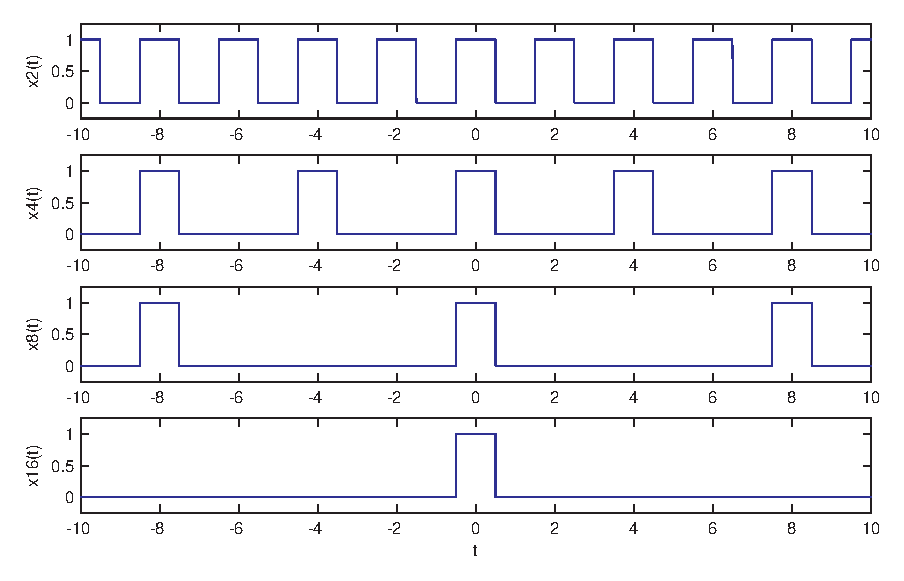
\includegraphics{fs2ft1}
\end{center}
Note that all versions of the signal have a unit pulse at the origin.  However, as $T$ increases the pulses neighbouring the center pulse move further and further from the origin.  In the limit as $T \to \infty$ only the central pulse remains, and the signal is no longer periodic.  This is the mechanism by which we can consider a frequency representation of aperiodic signals. 

The fundamental frequency is $\omega_0 = \frac{2 \pi}{T}$, which varies as $T$ changes.  The Fourier series representation of each instance of signal above is
\begin{equation*}
  x_T(t) = \sum_{k=-\infty}^{\infty} c_k e^{j k \frac{2 \pi}{T} t}
\end{equation*}
with Fourier series coefficients
\begin{equation*}
  c_k =  \begin{cases}
    \frac{1}{T} \qquad & k = 0 \\
    \frac{1}{k \pi} \sin \left( \frac{k \pi}{T} \right) \qquad & k \neq 0.
  \end{cases}  
\end{equation*}
As $T$ increases, the power of the signal drops and the Fourier series coefficients tend to zero.  However, the normalised product $T c_k$ has a special property, demonstrated below in terms of the magnitude:
\begin{center}
  \psfrag{-3pi}{\scriptsize $-3 \pi$}
  \psfrag{-2pi}{\scriptsize $-2 \pi$}
  \psfrag{-pi}{\scriptsize $-\pi$}
  \psfrag{pi}{\scriptsize $\pi$}
  \psfrag{2pi}{\scriptsize $2 \pi$}
  \psfrag{3pi}{\scriptsize $3 \pi$}
  \psfrag{0}{\scriptsize $0$}
  \psfrag{0.5}{\scriptsize $0.5$}
  \psfrag{1}{\scriptsize $1$}
  \psfrag{0}{\scriptsize $0$}
  \psfrag{w}{\scriptsize $\omega$}
  \psfrag{2|ck|}{\scriptsize $2 |c_k|$}
  \psfrag{4|ck|}{\scriptsize $4 |c_k|$}
  \psfrag{8|ck|}{\scriptsize $8 |c_k|$}
  \psfrag{16|ck|}{\scriptsize $16 |c_k|$}
  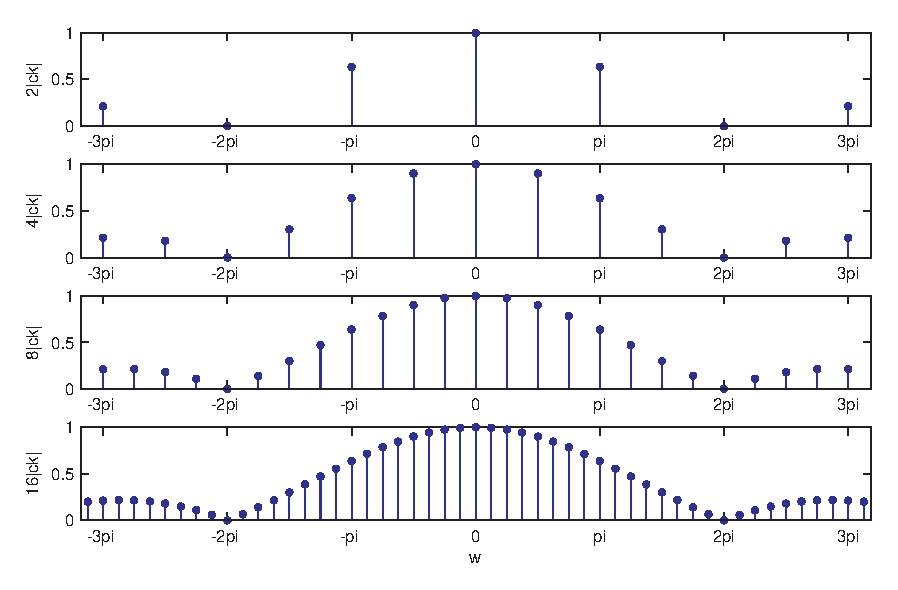
\includegraphics{fs2ft2}
\end{center}
As $T \to \infty$ the set of frequencies contained in the signal become more and more dense, passing into a continuum in the limit.  Note though that all the samples lie on an underlying curve $|X(\omega)|$ --- the magnitude of the Fourier transform of the isolated aperiodic pulse.

Formally, the forward and reverse Fourier transform can be defined as follows:
\begin{center}
\fbox{
\begin{minipage}{0.9\textwidth}
The Fourier transform {\em analysis} equation is:
\begin{equation*}
  X(\omega) = \int_{-\infty}^{\infty} x(t) e^{-j \omega t} dt
\end{equation*}
The {\em synthesis} equation is
\begin{equation*}
  x(t) = \frac{1}{2 \pi} \int_{-\infty}^{\infty} X(\omega) e^{j \omega t} d\omega.
\end{equation*}
A signal can be described either in the time domain (as a function of $t$) or in the frequency domain (as a function of $\omega$).  We often denote a Fourier transform pair as 
\begin{equation*}
  x(t) \quad \ftpair \quad X(\omega).
\end{equation*}
\end{minipage}
}
\end{center}
If $x(t)$ is absolutely integrable, so that
\begin{equation*}
  \int_{-\infty}^{\infty} |x(t)| dt < \infty
\end{equation*}
then the Fourier transform is guaranteed to exist.  However, a {\em generalised} Fourier transform can sometimes be defined even for signals that do not satisfy this property.

For a signal $x(t)$ the Fourier transform $X(\omega)$ is often also called the {\em frequency-domain representation} of $x(t)$, the {\em Fourier spectrum} of $x(t)$, or just the {\em spectrum} of $x(t)$.

The Fourier transform of the centered unit rectangular pulse can be found directly:
\begin{align*}
  X(\omega) &= \int_{-\infty}^{\infty} p_1(t) e^{-j \omega t} dt 
  = \int_{-1/2}^{1/2} e^{-j \omega t} dt 
  = \frac{1}{-j \omega} \left[ e^{-j \omega t} \right]_{t=-1/2}^{t=1/2} \\
  &= \frac{2j}{j \omega} \frac{1}{2j} (e^{j \omega 1/2} - e^{-j \omega 1/2})
  = \frac{2}{\omega} \sin (\omega/2).
\end{align*}
It is common to define the {\em sinc} function as follows:
\begin{equation*}
  \text{sinc}(x) = \frac{\sin(\pi x)}{\pi x},
\end{equation*}
so $\sin(\pi x) = \pi x \: \text{sinc}(x)$.  With $x = \frac{\omega}{2 \pi}$ the Fourier transform above can be written as
\begin{equation*}
  X(\omega) = \text{sinc} \left( \frac{\omega}{2 \pi} \right).
\end{equation*}
This is complex-valued function, so can be plotted in magnitude and phase form as below:
\begin{center}
  \psfrag{-3pi}{\scriptsize $-3 \pi$}
  \psfrag{-2pi}{\scriptsize $-2 \pi$}
  \psfrag{-pi}{\scriptsize $-\pi$}
  \psfrag{pi}{\scriptsize $\pi$}
  \psfrag{2pi}{\scriptsize $2 \pi$}
  \psfrag{3pi}{\scriptsize $3 \pi$}
  \psfrag{0}{\scriptsize $0$}
  \psfrag{0.5}{\scriptsize $0.5$}
  \psfrag{1}{\scriptsize $1$}
  \psfrag{0}{\scriptsize $0$}
  \psfrag{w}{\scriptsize $\omega$}
  \psfrag{|X(w)|}{\scriptsize $|X(\omega)|$}
  \psfrag{aX(w)}{\scriptsize $\angle X(\omega)$}
  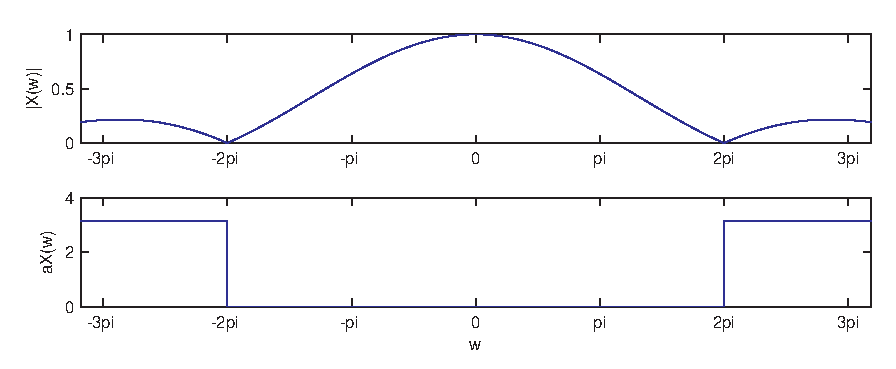
\includegraphics{fs2ft3}
\end{center}
Observe that $|X(\omega)|$ is the curve underlying the plots of $T |c_k|$ shown previously.

We have thus derived the following {\em Fourier transform pair}:
\begin{equation*}
  p_1(t) \quad \ftpair \quad \text{sinc} \left( \frac{\omega}{2 \pi} \right).
\end{equation*}

\subsection{Some Fourier transform pairs}

The signal $x(t) = e^{-b t} u(t)$ is absolutely integrable as long as $b>0$, since
\begin{equation*}
  \int_{-\infty}^{\infty} |e^{-b t} u(t)| dt = \int_0^{\infty} e^{-b t} dt
  = -\frac{1}{b} \left[ e^{-b t} \right]_{t=0}^{t=\infty} 
  = -\frac{1}{b} (0 - 1) = \frac{1}{b}
\end{equation*}
is then finite.  The ordinary Fourier transform of $x(t)$ is therefore guaranteed to exist.

In this case the Fourier representation of the signal $x(t) = e^{-b t} u(t)$ is given by
\begin{align*}
  X(\omega) &= \int_{-\infty}^{\infty} e^{-bt} u(t) e^{-j \omega t} dt
  = \int_{0}^{\infty} e^{(-b - j \omega) t} dt
  = \frac{1}{-b - j \omega} \left[ e^{(-b - j \omega) t} \right]_{t=0}^{t=\infty} \\
  &= - \frac{1}{b + j \omega} \left( \lim_{t \to \infty} e^{-bt} e^{j \omega t} - 1\right)
  = - \frac{1}{b + j \omega} \left( 0 - 1\right)
  = \frac{1}{b + j \omega}.
\end{align*}
The limit taken in this calculation can be justified as follows:  the complex number $e^{-bt} e^{j \omega t}$ is in polar form, with positive magnitude $e^{-bt}$.  As $t \to \infty$ this magnitude tends to zero, and the only complex quantity with magnitude zero is the number 0 itself.

Thus the following Fourier transform pair has been established:
\begin{equation*}
  e^{-bt} u(t) \quad \ftpair \quad \frac{1}{b + j \omega} \qquad \text{for} \qquad b>0.
\end{equation*}

Many signals of interest are not absolutely summable, and do not have a Fourier transform in the ordinary sense.  Take for example the very simple signal $x(t) = 1$, which is constant for all time.  This is about the most simple signal we can think of, but
\begin{equation*}
  \int_{-\infty}^{\infty} |x(t)| dt = \int_{-\infty}^{\infty} 1 dt \to \infty
\end{equation*}
and the sufficient condition for the existence is not met.  If we try to find
\begin{equation*}
  X(\omega) = \int_{-\infty}^{\infty} 1 e^{-j \omega t} dt
\end{equation*}
we will see that the integral doesn't converge.

Recalling that Fourier theory allows us to represent signals as additive combinations of scaled complex exponentials, we might expect that the signal $x(t) = 1$ only contains a component at frequency $\omega = 0$.  The Fourier transform $X(\omega) = 2 \pi \delta(\omega)$ is evidently related to this case.  What is the time-domain representation of this signal?  We can find it using the inverse transform:
\begin{align*}
  {\cal F}^{-1}\{X(\omega)\} &= \frac{1}{2 \pi} \int_{-\infty}^{\infty} X(\omega) e^{j \omega t} d\omega
  = \frac{1}{2 \pi} \int_{-\infty}^{\infty} 2 \pi \delta(\omega) e^{j \omega t} d\omega \\
  &= \int_{-\infty}^{\infty} \delta(\omega) e^{j 0 t} d\omega
  = \int_{-\infty}^{\infty} \delta(\omega) d\omega = 1.
\end{align*}
The {\em inverse} transform of $X(\omega) = 2 \pi \delta(\omega)$ is therefore $x(t) = 1$, even though the forward transform of $x(t)$ does not exist.  The pair
\begin{equation*}
  1 \quad \ftpair \quad 2 \pi \delta(\omega)
\end{equation*}
is valid in a generalised sense. 

This is analogous to the generalised derivative discussed earlier.  Finding the ordinary derivative $y(t)$ of a discontinuous signal $x(t)$ caused problems.  Instead we defined the generalised derivative as that signal $y(t)$ which, when integrated, resulted in the signal $x(t)$.  The generalised Fourier transform is similar.  We might not be able to find the Fourier transform $X(\omega)$ of a signal $x(t)$, but we could define the generalised transform of $x(t)$ to be that signal $X(\omega)$ which, when inverse transformed, yeilds $x(t)$.  In a sense a generalised Fourier pair is only valid in one direction --- but it causes no problems ignoring this distinction.

A similar but reverse situation arises when we consider the signal $x(t) = \delta(t)$.  The forward transform is 
\begin{equation*}
  X(\omega) = \int_{-\infty}^{\infty} \delta(t) e^{-j \omega t} dt
  = \int_{-\infty}^{\infty} \delta(t) e^{-j \omega 0} dt 
  = \int_{-\infty}^{\infty} \delta(t) dt = 1,
\end{equation*}
and we see that an impulse at the origin contains {\em equal} components of {\em all} possible frequencies.  The corresponding Fourier pair can be written as
\begin{equation*}
  \delta(t) \quad \ftpair \quad 1.
\end{equation*}
However, we cannot directly find the inverse transform of $X(\omega) = 1$ because the integral does not converge.  This is also a generalised Fourier pair.

Other transform pairs that are valid in a generalised context are
\begin{equation*}
  \delta(t - c) \quad \ftpair \quad e^{-j \omega c},
\end{equation*}
where the transform strictly only exists in the forward direction, and
\begin{equation*}
  e^{j \omega_0 t} \quad \ftpair \quad 2 \pi \delta(\omega - \omega_0),
\end{equation*}
where only the inverse transform is valid.

{\em Show\marginpar{\bf Exercise:} that the above two transform pairs are valid in a generalised context.}

From the last pair above, it is evident that the complex exponential $e^{j \omega_0 t}$ has the following spectrum:
\begin{center}
  \psfrag{w}{\scriptsize $\omega$}
  \psfrag{wc}{\scriptsize $\omega_c$}
  \psfrag{(2pi)}{\scriptsize $(2 \pi)$}
  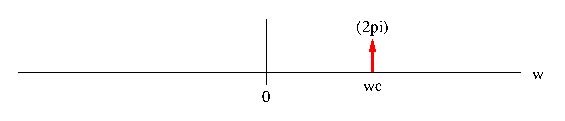
\includegraphics{compexpspectrum}
\end{center}
The {\em only} frequency present in this signal is at $\omega = \omega_0$.   When we talk about the component of a signal at frequency $\omega_0$ we mean the "amount" of $e^{j \omega_0 t}$ present in the signal, so this result should not be surprising.

Using the methods just outlined it is possible to identify a number of common Fourier transform pairs, tabulated below:
\begin{center}
\fbox{
\begin{minipage}{0.9\textwidth}
\doublespacing
\begin{center}
\begin{tabular}[h]{ll}
  %\hline
  $x(t) = \frac{1}{2\pi} \int_{-\infty}^{\infty} X(\omega) e^{j
    \omega t} d\omega \qquad$& 
  $X(\omega) = \int_{-\infty}^{\infty} x(t) e^{-j \omega t} dt$ \\
  \hline

  $1 \quad (-\infty < t < \infty)$ \hspace*{7ex} &
  $2 \pi \delta(\omega)$ \\

  $-0.5 + u(t)$ &
  $\frac{1}{j \omega}$ \\

  $u(t)$ &
  $\pi \delta(\omega) + \frac{1}{j \omega}$ \\

  $\delta(t)$ &
  $1$ \\

  $\delta(t-c)$ &
  $e^{-j \omega c} \quad (c \text{~any real number})$ \\

  $e^{-bt} u(t)$ &
  $\frac{1}{j \omega + b} \quad (b>0)$ \\

  $e^{j \omega_0 t}$ &
  $2\pi \delta(\omega - \omega_0) \qquad (\omega_0 \text{~any real
    number})$ \\

  $p_\tau(t)$ &
  $\tau \text{sinc} \frac{\tau \omega}{2\pi}$ \\

  $\tau \text{sinc} \frac{\tau t}{2\pi}$ &
  $2 \pi p_{\tau}(\omega)$ \\

  $\left( 1 - \frac{2|t|}{\tau} \right) p_\tau(t)$ &
  $\frac{\tau}{2} \text{sinc}^2 \left( \frac{\tau \omega}{4\pi}
  \right)$ \\

  $\frac{\tau}{2} \text{sinc}^2 \frac{\tau t}{4 \pi}$ &
  $2 \pi \left( 1 - \frac{2|\omega|}{\tau} \right) p_{\tau}(\omega)$ \\

  $\cos(\omega_0 t + \theta)$ &
  $\pi [ e^{-j \theta} \delta(\omega + \omega_0) +
  e^{j \theta} \delta(\omega - \omega_0) ]$ \\

  $\sin(\omega_0 t + \theta)$ &
  $j \pi [ e^{-j \theta} \delta(\omega + \omega_0) -
  e^{j \theta} \delta(\omega - \omega_0) ]$ \\

  %\hline
\end{tabular}
\end{center}
\end{minipage}
}
\end{center}
Using a table of transforms lets one use Fourier theory without having to formally manipulate integrals in every case.  

\subsection{Some Fourier transform properties}

There are a number of Fourier transform properties that can be applied to valid Fourier pairs to produce other valid pairs.  These properties often let us find Fourier transforms or inverse transforms without having to redo the integration every time.

Possibly the most important property is that the Fourier transform is linear.  To show what this means, suppose we have two valid Fourier pairs $x(t) \ftpair X(\omega)$ and $y(t) \ftpair Y(\omega)$.  The fact that these are valid pairs means that it must be the case that
\begin{equation*}
  X(\omega) = \int_{-\infty}^{\infty} x(t) e^{-j \omega t} dt \qquad \text{and} \qquad
  Y(\omega) = \int_{-\infty}^{\infty} y(t) e^{-j \omega t} dt.
\end{equation*}
Now consider the signal $z(t) = a x(t) + b y(t)$, where $a$ and $b$ are some constants.  It is a linear combination of the signals $x(t)$ and $y(t)$, for which we know the transforms.  What is the transform of $z(t)$?  By definition, 
\begin{align*}
  Z(\omega) &= \int_{-\infty}^{\infty} z(t) e^{-j \omega t} dt 
  = \int_{-\infty}^{\infty} (a x(t) + b y(t)) e^{-j \omega t} dt 
  = \int_{-\infty}^{\infty} (a x(t) e^{-j \omega t} + b y(t) e^{-j \omega t}) dt \\
  &= a \int_{-\infty}^{\infty} x(t) e^{-j \omega t} dt + b \int_{-\infty}^{\infty} y(t) e^{-j \omega t} dt
  = a X(\omega) + b Y(\omega).
\end{align*}
Thus we can obtain the frequency domain representation $Z(\omega)$ directly from the quantities $X(\omega)$ and $Y(\omega)$ --- it is also a linear combination with the same coefficients.  The property can be summarised as follows:
\begin{center}
\fbox{
\begin{minipage}{0.9\textwidth}
Linearity:
\begin{gather*}
  \text{If} \quad x(t) \ftpair X(\omega) \quad \text{and} \quad y(t) \ftpair Y(\omega), \\
  \text{then} \quad a x(t) + b y(t) \quad \ftpair \quad a X(\omega) + b Y(\omega).
\end{gather*}
\end{minipage}
}
\end{center}

How does the Fourier transform change if a signal is shifted in time?  Again, suppose we have a valid Fourier pair $x(t) \ftpair X(\omega)$, and consider the time-shifted signal $y(t) = x(t-c)$ for some constant $c$.  The frequency representation of $y(t)$ is 
\begin{align*}
  Y(\omega) &= \int_{-\infty}^{\infty} y(t) e^{-j \omega t} dt 
  = \int_{-\infty}^{\infty} x(t-c) e^{-j \omega t} dt
  = \int_{-\infty}^{\infty} x(p) e^{-j \omega (p+c)} dp \\
  &= e^{-j \omega c} \int_{-\infty}^{\infty} x(p) e^{-j \omega p} dp
  = e^{-j \omega c} X(\omega),
\end{align*}
where a change of variables $p = t-c$ has been made, and we observe that in the definition of the Fourier transform it doesn't matter what we call the dummy integration variable.  This result can be summarised as the following property:
\begin{center}
\fbox{
\begin{minipage}{0.9\textwidth}
Time shift:
\begin{align*}
  \text{If} \quad x(t) & \ftpair X(\omega) \\
  \text{then} \quad x(t-c) \quad & \ftpair \quad e^{-j \omega c} X(\omega).
\end{align*}
\end{minipage}
}
\end{center}
It is interesting to note that $|e^{-j \omega c} X(\omega)| = |X(\omega)|$, so shifting a signal in time doesn't change the amount of any frequency present;  only the phases of the different components changes.

Multiplying a signal by a complex exponential leads to another interesting Fourier transform property.  If $x(t) \ftpair X(\omega)$, then the transform of $y(t) = x(t) e^{j \omega_0 t}$ for some fixed value of $\omega_0$ is
\begin{align*}
  Y(\omega) &= \int_{-\infty}^{\infty} y(t) e^{-j \omega t} dt 
  = \int_{-\infty}^{\infty} x(t) e^{j \omega_0 t} e^{-j \omega t} dt 
  = \int_{-\infty}^{\infty} x(t) e^{-j (\omega - \omega_0) t} dt 
  = X(\omega - \omega_0).
\end{align*}
The property is as follows:
\begin{center}
\fbox{
\begin{minipage}{0.9\textwidth}
Frequency shift:
\begin{align*}
  \text{If} \quad x(t) & \ftpair X(\omega) \\
  \text{then} \quad x(t) e^{j \omega_0 t} \quad & \ftpair \quad X(\omega - \omega_0).
\end{align*}
\end{minipage}
}
\end{center}
Multiplying a signal by a complex exponential in time shifts the spectrum by $\omega_0$ in frequency.

Using similar methods one can prove a number of important other properties of the Fourier transform.  A summary is shown below.  Note that in all cases we assume that $x(t) \ftpair X(\omega)$ and $v(t) \ftpair V(\omega)$ are valid Fourier pairs:
\begin{center}
\fbox{
\begin{minipage}{0.9\textwidth}
\doublespacing
\begin{tabular}[h]{ll}
  %\hline
  Property & Transform Pair/Property \\
  \hline

  Linearity \hspace*{30ex} &
  $a x(t) + b v(t) \leftrightarrow a X(\omega) + b V(\omega)$ \\

  Time shift &
  $x(t-c) \leftrightarrow X(\omega) e^{-j \omega c}$ \\

  Time scaling &
  $x(at) \leftrightarrow \frac{1}{a} X(\frac{\omega}{a}) \quad a>0$ \\

  Time reversal &
  $x(-t) \leftrightarrow X(-\omega) = \overline{X(\omega)}$ \\

  Multiplication by power of $t$ &
  $t^n x(t) \leftrightarrow j^n \frac{d^n}{d \omega^n} X(\omega) \quad
  n=1,2,\ldots$ \\

  Frequency shift &
  $x(t) e^{j \omega_0 t} \leftrightarrow X(\omega - \omega_0) \quad
  \omega_0 \text{~real}$ \\

  Multiplication by $\cos(\omega_0 t)$ &
  $x(t) \cos(\omega_0 t) \leftrightarrow \frac{1}{2} [ X(\omega +
  \omega_0) + X(\omega - \omega_0) ]$ \\

  Differentiation in time domain &
  $\frac{d^n}{d t^n} x(t) \leftrightarrow (j \omega)^n X(\omega) \quad
  n=1,2,\ldots$ \\

  Integration &
  $\int_{-\infty}^t x(\lambda) d\lambda \leftrightarrow \frac{1}{j
    \omega} X(\omega) + \pi X(0) \delta(\omega)$ \\

  Convolution in time domain &
  $x(t) \conv v(t) \leftrightarrow X(\omega) V(\omega)$ \\

  Multiplication in time domain &
  $x(t) v(t) \leftrightarrow \frac{1}{2\pi} X(\omega) \conv V(\omega)$
  \\

  Parseval's theorem &
  $\int_{-\infty}^{\infty} x(t) v(t) dt = \frac{1}{2\pi}
  \int_{-\infty}^{\infty} \overline{X(\omega)} V(\omega) d\omega$ \\

  Parseval's theorem (special case) &
  $\int_{-\infty}^{\infty} x^2(t) dt = \frac{1}{2\pi}
  \int_{-\infty}^{\infty} |X(\omega)|^2 d\omega$ \\

  Duality &
  $X(t) \leftrightarrow 2\pi x(-\omega)$ \\

  %\hline
\end{tabular}
\end{minipage}
}
\end{center}

Using the transform properties is easy.  Take any valid Fourier transform pair $x(t) \ftpair X(\omega)$, say
\begin{equation*}
  e^{-bt} u(t) \quad \ftpair \quad \frac{1}{b + j \omega} \quad \text{for} \quad b>0.
\end{equation*}
In this case we have $x(t) = e^{-bt} u(t)$ and $X(\omega) = \frac{1}{b + j \omega}$.  The duality property, for example, states that
\begin{equation*}
  X(t) \quad \ftpair \quad 2 \pi x(-\omega)
\end{equation*}
is also a valid Fourier pair.  By simply writing the implication in terms of the quantities defined, we obtain the new pair
\begin{equation*}
  \frac{1}{b + j t} \quad \ftpair \quad 2 \pi e^{-b(-\omega)} u(-\omega) \quad \text{for} \quad b>0.
\end{equation*}
Duality effectively lets us swap the expressions for signals between the time and the frequency domains.

To use standard transform pairs and properties to find the Fourier transform of a more complicated time-domain signal may require some insight.  The principle is simple, though:  apply a sequence of transform properties to appropriately selected known pairs, until the left-hand side equals the quantity you're trying to transform.  The right-hand side then provides the solution.

{\em Example:}  Suppose we need to find the Fourier transform of the signal $y(t) = e^{-2t} u(t-2) e^{j 3 t}$.  

One way to proceed is to notice that multiplication by $e^{j 3 t}$ in time corresponds to a frequency shift.  Thus if we knew the transform of $e^{-2t} u(t-2)$ we could easily obtain the answer.  Now 
\begin{equation*}
  e^{-2t} u(t-2) = e^{-4} e^4 e^{-2t} u(t-2) = e^{-4} e^{-2(t-2)} u(t-2),
\end{equation*}
and since $e^{-4}$ is a constant we only need to know the transform of $e^{-2(t-2)} u(t-2)$.  This can be obtained by applying a time shift to $e^{-2t} u(t)$.  To construct the original signal we can therefore start with $e^{-2t} u(t)$, apply a time shift to get $e^{-2(t-2)} u(t-2)$, then apply scaling to get $e^{-4} e^{-2(t-2)} u(t-2) = e^{-2t} u(t-2)$, and finally frequency shift the result to get $e^{-2t} u(t-2) e^{j 3 t}$.

A formal solution can therefore be obtained as follows.  (One need not answer questions with such rigour.)  Start with the valid Fourier pair
\begin{equation*}
  e^{-2t} u(t) \quad \ftpair \quad \frac{1}{2 + j \omega}.
\end{equation*}
\begin{enumerate}

\item The time shift property for $c-2$ states that if $x(t) \ftpair X(\omega)$ is a valid pair then
\begin{equation*}
  x(t-2) \quad \ftpair \quad X(\omega) e^{-j \omega 2}
\end{equation*}
is also a valid pair.  Letting $x(t) = e^{-2t} u(t)$ and $X(\omega) = \frac{1}{2 + j \omega}$ this yields the new Fourier transform pair
\begin{equation*}
  e^{-2(t-2)} u(t-2) \quad \ftpair \quad  \frac{1}{2 + j \omega} e^{-j \omega 2}.
\end{equation*}

\item The linearity property states that
\begin{equation*}
  a x(t) + b v(t) \quad \ftpair \quad a X(\omega) + b V(\omega)
\end{equation*}
for any $x(t) \ftpair X(\omega)$ and $v(t) \ftpair V(\omega)$.  For $a = e^{-4}$ and $b=0$ this becomes
\begin{equation*}
  e^{-4} x(t) \quad \ftpair \quad e^{-4} X(\omega).
\end{equation*}
Letting $x(t) =  e^{-2(t-2)} u(t-2)$ and $X(\omega) = \frac{1}{2 + j \omega} e^{-j \omega 2}$ therefore gives the new pair
\begin{equation*}
   e^{-4} e^{-2(t-2)} u(t-2) \quad \ftpair \quad  e^{-4} \frac{1}{2 + j \omega} e^{-j \omega 2}.
\end{equation*}

\item The frequency shift property states that if $x(t) \ftpair X(\omega)$ is a valid pair then
\begin{equation*}
  x(t) e^{j 3 t} \quad \ftpair \quad X(\omega - 3)
\end{equation*}
is also a valid pair.  With $x(t) =  e^{-4} e^{-2(t-2)} u(t-2)$ and $X(\omega) = e^{-4} \frac{1}{2 + j \omega} e^{-j \omega 2}$ this yields
\begin{equation*}
   e^{-4} e^{-2(t-2)} u(t-2) e^{j 3 t} \quad \ftpair \quad   e^{-4} \frac{1}{2 + j (\omega-3)} e^{-j (\omega-3) 2}.
\end{equation*}

\end{enumerate}

Since the left-hand side is the quantity we were looking for the transform of, the right-hand side must be the required transform:
\begin{equation*}
  Y(\omega) = e^{-4} \frac{1}{2 + j (\omega-3)} e^{-j (\omega-3) 2}.
\end{equation*}

Finding the inverse transform of a signal is similar, except we need to determine a set of pairs and properties that can be combined to give the required frequency domain expression.

\subsection{Convolution property}

Possibly the most important property of the Fourier transform relates to time-domain convolution.  According to this property, if $x(t) \ftpair X(\omega)$ and $v(t) \ftpair V(\omega)$, then
\begin{equation*}
  x(t) \conv v(t) \quad \ftpair \quad X(\omega) V(\omega).
\end{equation*}
It is much easier to think about {\em multiplying} two signals together than it is to think of {\em convolution}.  Note, though, that mathematically they are the {\em same} operation.  The Fourier transform simply represents the signals $x(t)$ and $v(t)$ in a form where convolution becomes much simpler.

To see how this property comes about, it is useful to think about the relationship in terms of a system and its impulse response.  The convolution $y(t) = x(t) \conv v(t)$ can be thought of as the output of a system with impulse response $v(t)$ when the input is $x(t)$.  It was shown previously that for the special case where the input is $x(t) = e^{j \omega t}$ the output will be $y(t) = V(\omega) e^{j \omega t}$:  this is the defining property of how systems respond to frequencies.  The following input-output pair is therefore valid for the system
\begin{equation*}
  e^{j \omega t} \longrightarrow V(\omega) e^{j \omega t},
\end{equation*}
for all values of $\omega$.  Therefore $v(t) \conv e^{j \omega t} = V(\omega) e^{j \omega t}$.

Note now that $x(t)$ can be written in terms of the inverse Fourier transform as
\begin{equation*}
  x(t) = \frac{1}{2 \pi} \int_{-\infty}^{\infty} X(\omega) e^{j \omega t} d\omega.
\end{equation*}
Since convolution is a linear operation, the following is seen to hold:
\begin{align*}
  y(t) &= v(t) \conv x(t) 
  = v(t) \conv \left( \frac{1}{2 \pi} \int_{-\infty}^{\infty} X(\omega) e^{j \omega t} d\omega \right)
  = \frac{1}{2 \pi} v(t) \conv \left( \int_{-\infty}^{\infty} X(\omega) e^{j \omega t} d\omega \right) \\
  &= \frac{1}{2 \pi} \int_{-\infty}^{\infty} v(t) \conv \left( X(\omega) e^{j \omega t} \right) d\omega 
  = \frac{1}{2 \pi} \int_{-\infty}^{\infty} X(\omega) \left( v(t) \conv e^{j \omega t} \right) d\omega \\
  &= \frac{1}{2 \pi} \int_{-\infty}^{\infty} X(\omega) V(\omega) e^{j \omega t} d\omega 
\end{align*}
But from the definition of the inverse Fourier transform 
\begin{equation*}
  y(t) = \frac{1}{2 \pi} \int_{-\infty}^{\infty} Y(\omega) e^{j \omega t} d\omega,
\end{equation*}
so we see that $Y(\omega) = X(\omega) V(\omega)$.

{\em Example:}  Find $y(t) = x(t) \conv v(t)$ where $x(t) = e^{-t} u(t)$ and $v(t) = e^{-2t} u(t)$ using frequency-domain methods.

The equivalence of convolution in time and multiplication in frequency means that $Y(\omega) = X(\omega) V(\omega)$.  However, from tables we see that
\begin{equation*}
  X(\omega) = \frac{1}{1 + j \omega} \qquad \text{and} \qquad
  V(\omega) = \frac{1}{2 + j \omega},
\end{equation*}
so
\begin{equation*}
  Y(\omega) = \frac{1}{(1 + j \omega)(2 + j \omega)} 
\end{equation*}
Using a partial fraction expansion this becomes
\begin{equation*}
  = \frac{A}{1 + j \omega} + \frac{B}{2 + j \omega},
\end{equation*}
with $A=1$ and $B=-1$ (maybe?).  The inverse Fourier transform gives the required solution:
\begin{equation*}
  y(t) = e^{-t} u(t) - e^{-2t} u(t).
\end{equation*}

\subsection{Solving linear constant coefficient differential equations}

Previously it was stated that any system that has an input-output relation governed by a LCCDE is linear and time invariant.  It therefore has an impulse response that completely describes its behaviour in terms of time domain convolution.  Fourier methods provide a simple way of finding this impulse response.

Suppose a system's input-output relation is described by 
\begin{equation*}
  x(t) = y(t) + 2 \frac{d}{dt} y(t).
\end{equation*}
We can substitute any given input $x(t)$ into this expression, and solve for the resulting output $y(t)$ (in this case up to a single undetermined constant, since it is a first-order differential equation in $y(t)$).  Denoting the impulse response by $h(t)$, and noting that it is just the output when the input is $x(t) = \delta(t)$, we see that the impulse response can be found by solving the differential equation
\begin{equation*}
  \delta(t) = h(t) + 2 \frac{d}{dt} h(t).
\end{equation*}
While this expression is true, it doesn't provide a simple means of finding $h(t)$.

The differentiation in time property can be used to express the system LCCDE in the frequency domain as
\begin{equation*}
  X(\omega) = Y(\omega) + 2 j \omega Y(w) = Y(\omega) [1 + j 2 \omega]
\end{equation*}
Since $Y(\omega) = H(\omega) X(\omega)$, we can find the transfer function of the system as follows:
\begin{equation*}
  H(\omega) = \frac{Y(\omega)}{X(\omega)} = \frac{1}{1 + j 2 \omega}
  = \frac{1/2}{1/2 + j \omega}.
\end{equation*}
The impulse response is just the inverse Fourier transform of the transfer function:
\begin{equation*}
  h(t) = {\cal F}^{-1} \{ H(\omega) \} = \frac{1}{2} e^{-\frac{1}{2} t} u(t).
\end{equation*}
A differential equation in the time domain becomes an algebraic equation in the frequency domain.

Notice that the solution obtained in this manner does not include the undetermined constant that one would expect from solving a first-order differential equation.  There is an implicit assumption that gets made in terms of initial conditions when using the Fourier transform to obtain the solution.  Usually this is not a concern to us, but if a more formal solution is required then the {\em Laplace transform} is a more appropriate tool.  The Laplace transform is essentially an extended Fourier transform that is able to do transient analysis of LCCDEs.

\subsection{Link between Fourier series and Fourier transform}

It turns out that there's only really one Fourier series that is important, namely that of the impulse train $p(t)$ below:
\begin{center}
  \psfrag{t}{\scriptsize $t$}
  \psfrag{T}{\scriptsize $T$}
  \psfrag{(1)}{\scriptsize $(1)$}
  \psfrag{p(t)}{\scriptsize $p(t)$}
  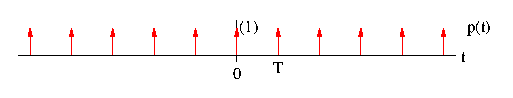
\includegraphics{imptraintfp}
\end{center}
We could write this signal as $p(t) = \sum_{k=-\infty}^{\infty} \delta(t - kT)$, but since it is clearly periodic it's more useful to express it as a Fourier series
\begin{equation*}
  p(t) = \sum_{k=-\infty}^{\infty} c_k e^{j k \omega_s t} \qquad \text{with} \qquad \omega_s = \frac{2 \pi}{T}.
\end{equation*}
The coefficients are particularly simple to calculate:
\begin{equation*}
  c_k = \frac{1}{T} \int_{-T/2}^{T/2} \delta(t) e^{-j k \omega_s t} dt = 
  \frac{1}{T} \int_{-T/2}^{T/2} \delta(t) e^{-j k \omega_s (0)} dt = \frac{1}{T}
\end{equation*}
Thus we can write $p(t) = \sum_{k=-\infty}^{\infty} \frac{1}{T} e^{j k \omega_s t}$.

The Fourier transform of this expression can be used to find the signal in the frequency domain:
\begin{equation*}
  P(\omega) = {\cal F}\{p(t)\} 
  = \sum_{k=-\infty}^{\infty} \frac{1}{T} {\cal F}\{ e^{j k \omega_s t} \}
  = \sum_{k=-\infty}^{\infty} \frac{2 \pi}{T} \delta(\omega - k \omega_s)
  = \sum_{k=-\infty}^{\infty} \omega_s \delta(\omega - k \omega_s).
\end{equation*}
This is also a sequence of impulses, but in the frequency domain --- an impulse train in time transforms to an impulse train in frequency.  This can be depicted by the transform pair below:
\begin{center}
  \psfrag{t}{\scriptsize $t$}
  \psfrag{w}{\scriptsize $\omega$}
  \psfrag{T}{\scriptsize $T$}
  \psfrag{(1)}{\scriptsize $(1)$}
  \psfrag{(ws)}{\scriptsize $(\omega_s)$}
  \psfrag{ws}{\scriptsize $\omega_s$}
  \psfrag{p(t)}{\scriptsize $p(t)$}
  \psfrag{P(w)}{\scriptsize $P(\omega)$}
  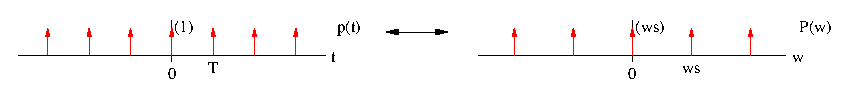
\includegraphics{imptraintf}
\end{center}
or
\begin{equation*}
  \sum_{k=-\infty}^{\infty} \delta(t - kT) \quad \ftpair \quad 
  \frac{2 \pi}{T} \sum_{k=-\infty}^{\infty} \delta(\omega - k \omega_s) \quad \text{with} \quad \omega_s = \frac{2 \pi}{T}.
\end{equation*}
If we choose a small value of $T$, so that the impulses are close together in time, then the spacing $\omega_s = \frac{2 \pi}{T}$ in the frequency domain is large.

We can use this result to find the Fourier series of a periodic signal, and demonstrate by example.

{\em Example:}  Suppose we want the Fourier series representation of the signal below:
\begin{center}
  \psfrag{1/2}{\scriptsize $\frac{1}{2}$}
  \psfrag{1}{\scriptsize $1$}
  \psfrag{-1}{\scriptsize $-1$}
  \psfrag{t}{\scriptsize $t$}
  \psfrag{x(t)}{\scriptsize $x(t)$}
  
\includegraphics{exampleftfs}
\end{center}
Because $x(t)$ is periodic (with a period $T=2$) we can write it as the convolution of $p(t)$ and $z(t)$ as shown below:
\begin{center}
  \psfrag{1/2}{\scriptsize $\frac{1}{2}$}
  \psfrag{2}{\scriptsize $2$}
  \psfrag{(1)}{\scriptsize $(1)$}
  \psfrag{t}{\scriptsize $t$}
  \psfrag{z(t)}{\scriptsize $z(t)$}
  \psfrag{p(t)}{\scriptsize $p(t)$}
  \psfrag{*}{$\conv$}
  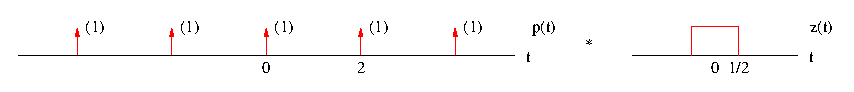
\includegraphics{exampleftfsdec}
\end{center}
Convolution $x(t) = p(t) \conv z(t)$ in time is multiplication $X(\omega) = P(\omega) Z(\omega)$ in frequency.  Also, since $z(t) = p_1(t)$ we know from standard transform tables that $Z(\omega) = \text{sinc} \left( \frac{\omega}{2\pi} \right)$.  The transform of $x(t)$ can therefore be written as
\begin{equation*}
  X(\omega) = P(\omega) Z(\omega) = \left( \pi \sum_{k=-\infty}^{\infty} \delta(\omega - k \pi) \right) Z(\omega)
  = \pi \sum_{k=-\infty}^{\infty} Z(k \pi) \delta(\omega - k \pi),
\end{equation*}
where the sifting or sampling property of the delta function has been used.  Inverting to the time domain gives
\begin{equation*}
  x(t) = \sum_{k=-\infty}^{\infty} \frac{Z(k \pi)}{2} e^{j k \pi t},
\end{equation*}
which is exactly in the form of a Fourier series $x(t) = \sum_{k=-\infty}^{\infty} c_k e^{j k \pi t}$ with $c_k = Z(k \pi)/2$.  The series coefficients are therefore $c_0 = 1/2$ and
\begin{equation*}
  c_k = \frac{1}{2} \text{sinc} \left( \frac{k\pi}{2\pi} \right)
  = \frac{1}{2} \text{sinc} \left( \frac{k}{2} \right) = \frac{1}{k \pi} \sin \left( \frac{k \pi}{2} \right)
\end{equation*}
for $k \neq 0$.  This is the same as the result that would be obtained using direct integration to get the coefficients.

%\subsection{Modulation}
%[put this somewhere else?]
%
%Modulation property and telecomms example?

\end{document}
